%%%%%%%%%%%%%%%%%%%%%% PREAMBULE %%%%%%%%%%%%%%%%%%%%%%%%%%%%%%%%%%%%%%%%

%%%%%%%%%%%%%%%% PARAMETRES DU DOCUMENT %%%%%%%%%%%%%%%%%%%%%%%%%%%%%%%%%
\documentclass[12pt,a4paper]{article}
\usepackage[utf8]{inputenc}
\usepackage[T1]{fontenc}
\usepackage[french]{babel}

%%%%%%%%%%%%%%%%%%%%% PACKAGES %%%%%%%%%%%%%%%%%%%%%%%%%%%%%%%%%%%%%%%%%%
\usepackage{hyperref}
\usepackage{shorttoc}
\setlength{\parindent}{0pt}
\usepackage[top=2cm,bottom=2cm,right=2cm,left=2cm]{geometry}
\usepackage{multicol}
\usepackage{nccrules}
\usepackage{eurosym}
\usepackage{listings}
\usepackage{caption}
\usepackage{makecell}
\usepackage{graphicx}
\usepackage{subfigure}
\usepackage{hyperref}
\usepackage{biblatex}
\addbibresource{biblio.bib}

%%%%%%%%%%%%%%%%%%%%%%%%%%%%%%%%%%%%%%%%%%%%%%%%%%%%%%%%%%%%%%%%%%%%%%%%%


%%%%%%%%%%%%%%% PARAMETRAGES PACKAGES %%%%%%%%%%%%%%%%%%%%%%%%%%%%%%%%%%%
\captionsetup{labelformat=empty}

\hypersetup{
	colorlinks=true,
	linkcolor=blue,
	urlcolor=blue,
	citecolor=black
	}
	
\usepackage[
    left = \flqq{},% 
    right = \frqq{},% 
    leftsub = \flq{},% 
    rightsub = \frq{} %
]{dirtytalk}

%%%%%%%%%%%%%%%%%%%%%%%%%%%%%%%%%%%%%%%%%%%%%%%%%%%%%%%%%%%%%%%%%%%%%%%%%

\setlength{\fboxrule}{.2pt}

%%%%% PAGE DE TITRE %%%%
\title{Groupe F - Synthèse}

\author{Hudayfa Koujdal - Hugo Lignères - Soukaina Mourabit - Samantha Ortega}

\date{UE L315 - Semaine 4}

\begin{document}

\maketitle

\hrulefill
\vspace{6cm}
\begin{center}
	
\includegraphics[scale=.4]{../images/univ.png}
		\\
		\vspace{2cm}
	
\includegraphics[scale=.25]{../images/cvtic.png}
\end{center}

%%%%%%%%%%%%%%%%%%%%%%%%%%%%%%%%%%%%%%%%%%%%%%%%%%%%%%%%%%%%%%%%%%%%%%%%%%
\newpage

\tableofcontents

\newpage

\section{Introduction}

Pour ce mini-projet, nous devions implémenter une médiathèque, qui permet à un utilisateur d'emprunter et de rendre les documents affichés. 

Les données à utiliser proviennent d'une collection \say{\texttt{documents}}, stockée dans une base de données de type NoSQL, elle-même hébergée dans un cluster MongoDB Atlas. 


Pour créer la logique de l'application et interagir avec les données de la collection, nous avons utilisé Node.js avec le framework Express.js. \\

Nous allons d'abord voir comment nous nous sommes organisés pour ce travail de groupe. Puis, dans une deuxième partie, nous reviendrons sur ce que nous avons produit. Enfin, en conclusion, chaque membre du groupe fera un retour d'expérience.

\section{Organisation générale}

	\subsection{Répartition du travail}
	
Pour ce projet, nous avons décidé de répartir les rôles de cette manière : \\

\begin{table}[!h]
	\centering
		\begin{tabular}{|c|l|}
			\hline
			& \\
			\textbf{Nom} & \textbf{Mission} \\ 
			& \\\hline
			& \\
			\textbf{Hugo} & \makecell[l]{\textbf{- Affichage des documents :} \\ \hspace{.5cm} - Création de l'interface pour afficher les documents ; \\ \hspace{.5cm} - Affichage des informations principales (titre, auteur, etc.) ; \\ \textbf{- Mise en place du projet et du dépôt GitHub} \\ \textbf{- Rédaction du rapport}}\\ 
			& \\ \hline
			& \\
			\textbf{Samantha} & \makecell[l]{\textbf{- Emprunt et retour des documents :} \\ \hspace{.5cm} - Création de fonctionnalités pour emprunter et rendre des documents \\ \hspace{.5cm} - Mise en place d'un mécanisme pour suivre le statut d'un document } \\ 
			& \\ \hline
			& \\
			\textbf{Soukaina} & \makecell[l]{ \textbf{- Gestion des utilisateurs: }\\ \hspace{.5cm} - Implémentation du système d'authentification ;\\ \hspace{.5cm} - Gestion de la connexion des utilisateurs.}\\ 
			& \\ \hline
			& \\
			\textbf{Hudayfa} & \makecell[l]{ \textbf{- Rôle administrateur :} \\  \hspace{.5cm}- Création de l'interface d'administration (ajout, suppression) ; \\ \hspace{.5cm}- Création de l'interface de gestion des documents (ajouter, supprimer).} \\
			& \\ \hline
		\end{tabular}
	\caption{Répartition des rôles au sein du groupe}
\end{table}	

\newpage
		
	\subsection{Méthode d'organisation}
	
	Pour le dépôt GitHub, nous avons utilisé la fonctionnalité des branches pour faciliter le travail en asynchrone. Nous nous sommes mis d'accord pour que ces branches doivent respecter la nomenclature suivante : \texttt{"nom\_fonctionnalité"}. Par exemple, \texttt{"hudayfa\_admin"} ou \texttt{"soukaina\_auth"}. 
	
	Pour la communication interne, nous avons décidé d'utiliser l'outil Teams. Nous y avons intégré un cahier de bord, pour que chaque membre puisse y noter tous les changements apportés au projet.
	


		
		\subsection{Dépôt GitHub du projet}
		
		 \textit{\href{https://github.com/hugolgs-dev/l315-semaine-4-groupe-f}{Lien vers le dépôt du projet}} \\
		 
\begin{figure}[!h]
	\begin{center}
		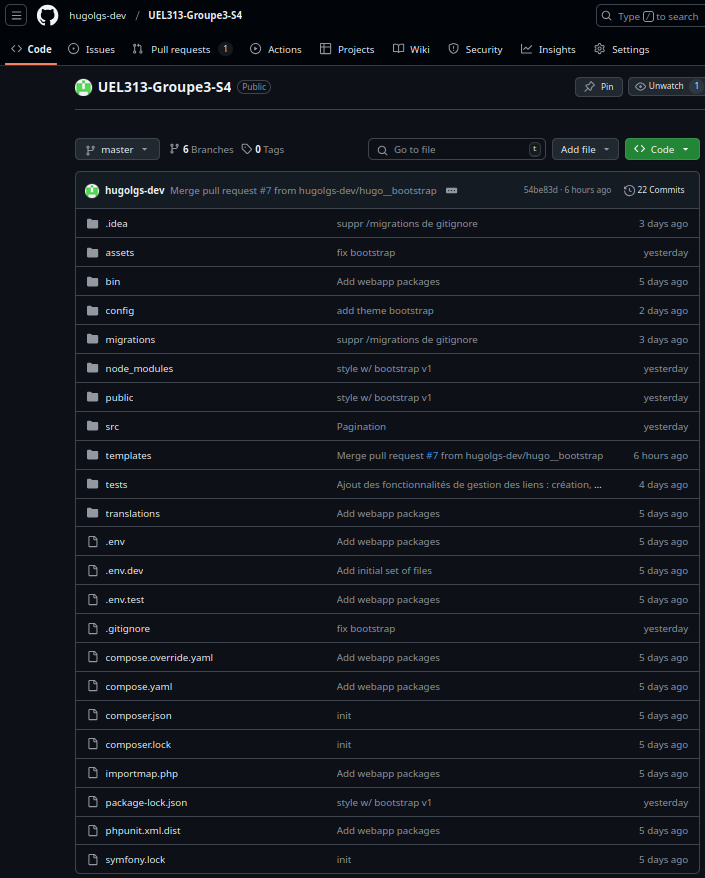
\includegraphics[scale=.9]{depot.png}
		\caption{Dépôt GitHub du projet}
	\end{center}
\end{figure}	

\newpage

Une rapide explication des principaux répertoires du projet et de leur rôles : \\
		 
		 \begin{itemize}
			
			\item \texttt{Controllers/AuthController.js} $\rightarrow$ On trouve dans ce fichier les fonctions qui gèrent l'authentification des utilisateurs ( \texttt{signUp(), login(), logout()}).
			
			\item \texttt{models} $\rightarrow$ C'est dans ce répertoire que se trouvent les fichiers de schémas de données utilisés par MongoDB via l'ORM Mongoose. 
			
			\item \texttt{routes/index.js} $\rightarrow$ C'est ici que les routes de l'application sont définies.
			
			\item \texttt{views} $\rightarrow$ Dans ce répertoire se trouvent les fichiers de vues, qui utilisent le moteur de templates \texttt{EJS} pour générer le contenu des pages dans le navigateur. \\
		
		 \end{itemize} 
		 
Il y a également les fichiers \texttt{app.js} et \texttt{start.js}. Le premier permet de configurer les différents éléments du projet: Express.js, les templates EJS, les routes, et les fichiers BootStrap. La ligne \texttt{module.exports = app;} permet d'utiliser ces éléments configurés dans tout le code de l'application.

Le deuxième est responsable de la connexion à la base de données et du démarrage du serveur Express.

			
\newpage

\section{Fonctionnalités implémentées}

Dans cette partie, nous allons aborder les principales fonctionnalités implémentées, ainsi que certaines parties importantes du code.

\subsection{Affichage et emprunt des documents}

Ces fonctionnalités permettent d'afficher les documents et de gérer les emprunts et les retours de documents en utilisant Express, Mongodb et EJS. Plusieurs routes ont été mises en place :  \\

\begin{itemize}
	\item \texttt{GET /documents} pour afficher tous les documents disponibles 
	\item \texttt{POST /emprunter/:id} pour emprunter un document 
	\item \texttt{POST /rendre/:id} pour retourner un document. \\
\end{itemize} 

 Un middleware d'authentification a été intégré afin de restreindre certaines actions aux utilisateurs connectés.
Dans les vues EJS, l'affichage a été adapté pour que tous les utilisateurs puissent voir les documents, mais que seul un utilisateur connecté puisse emprunter un document. Les documents empruntés s'affichent uniquement pour l'utilisateur concerné. Un champ \texttt{emprunteur} a été ajouté dans la base de données afin d’associer chaque emprunt à un utilisateur spécifique.

\begin{figure}[!h]
	\begin{center}
		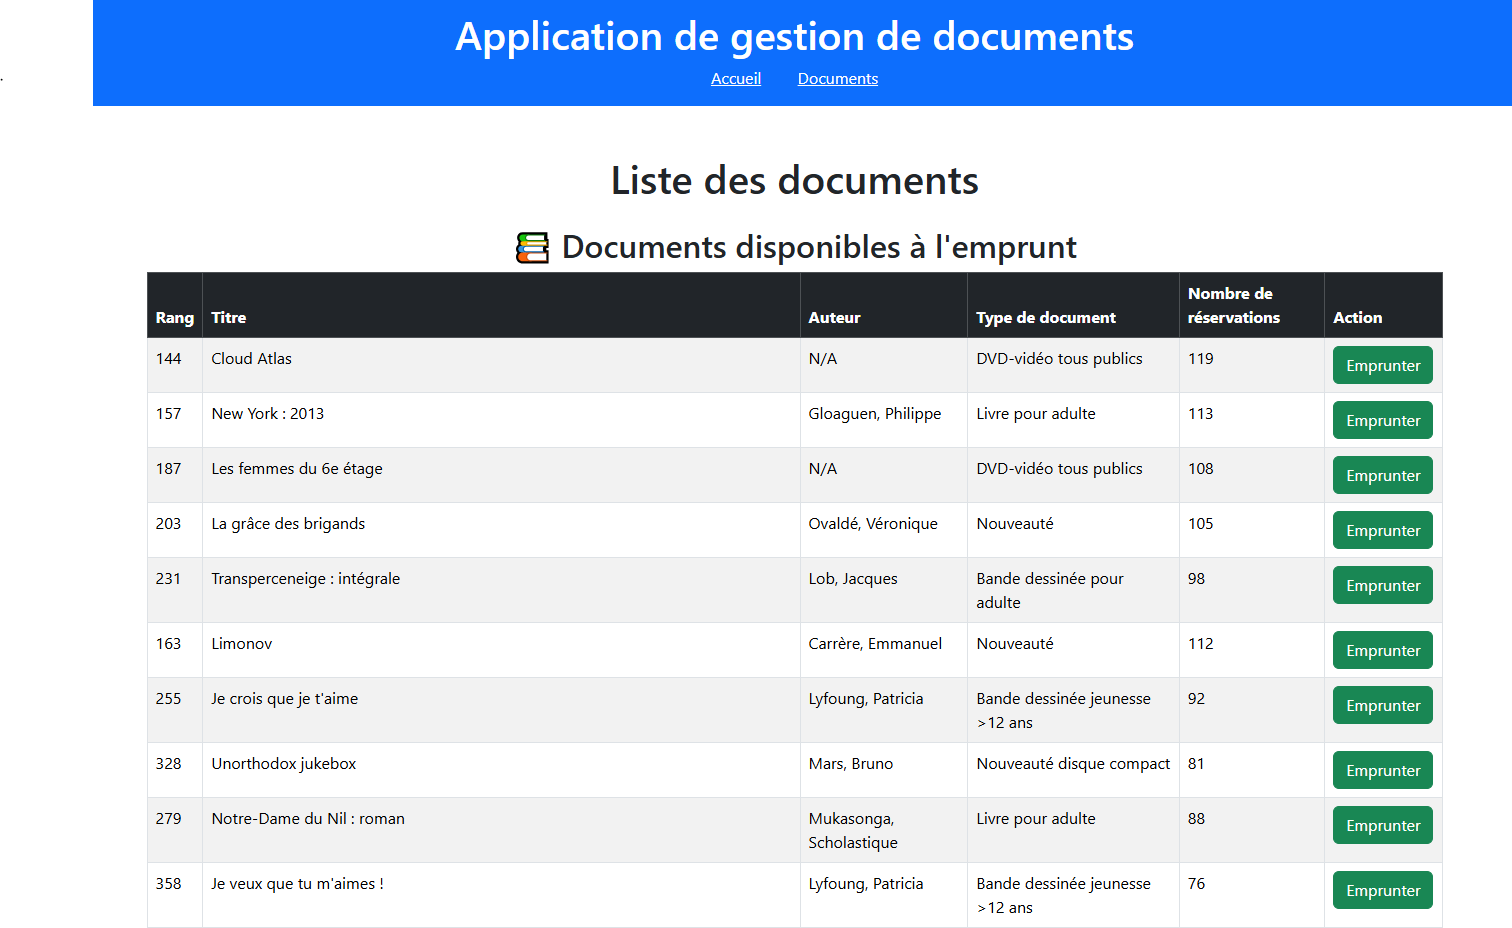
\includegraphics[scale=.3]{affichage_emprunt.png}
		\caption{Page d'affichage des documents disponibles à l'emprunt} 
	\end{center}
\end{figure}

\begin{figure}[!h]
	\begin{center}
		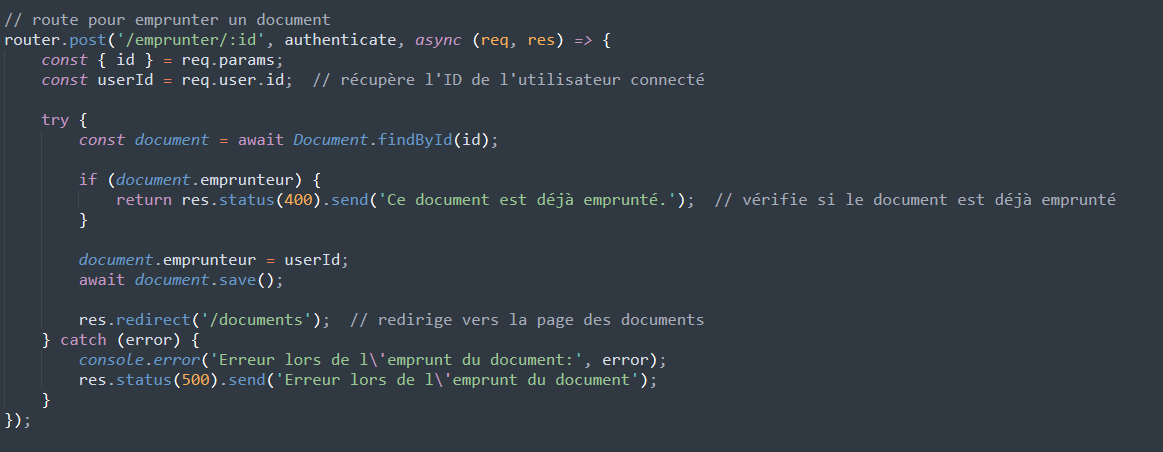
\includegraphics[scale=.4]{route_emprunt.png}
		\caption{Exemple de route}
	\end{center}
\end{figure}

\newpage
%\subsection{Inscription des utilisateurs}

%Dans un premier temps, il a fallu créer un modèle utilisateur

%\begin{figure}[!h]
%	\begin{center}
%		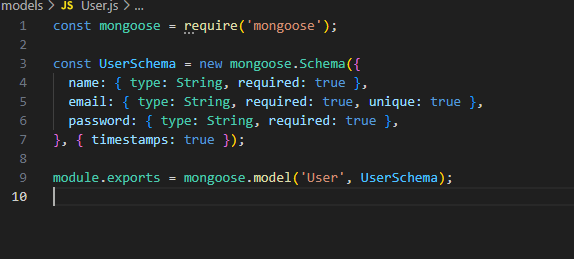
\includegraphics[scale=1]{userjs.png}
%		\caption{User.js}
%	\end{center}
%\end{figure}

%\subsection{Connexion et deconnexion}

\subsection{Interface administration}

Le travail a consisté à implémenter un système d'authentification pour un administrateur et à ajouter des fonctionnalités de gestion des utilisateurs et des documents. Le modèle \texttt{Admin} a été créé avec un hachage du mot de passe, et le contrôleur \texttt{AdminAuthController} gère l'inscription, la connexion et la déconnexion.\\

Des routes ont été ajoutées au fichier \texttt{index.js} pour permettre à l'administrateur de s'inscrire, de se connecter et de se déconnecter, ainsi que pour ajouter  et supprimer des utilisateurs et des documents, qui sont : \\

\begin{itemize}
	\item \texttt{POST /admin/add-user} ;
	\item \texttt{POST /admin/add-document} ;
	\item \texttt{DELETE /admin/delete-user/:id} ;
	\item \texttt{DELETE /admin/delete-document/:id}. \\
\end{itemize}

Les vues ont été mises à jour pour refléter ces fonctionnalités : \texttt{admin/dashboard.ejs} permet la gestion des utilisateurs et des documents, tandis que \texttt{admin/login.ejs} et \texttt{admin/signup.ejs} offrent des interfaces pour la connexion et l'inscription des administrateurs. Le header a été modifié pour inclure un lien vers la page de connexion, facilitant l'accès. Ce système offre une gestion sécurisée et efficace du contenu pour l'administrateur. \\

\newpage

Voici le rendu sur la page d'administration : 

\begin{figure}[!h]
	\begin{center}
		\setlength{\fboxsep}{0pt}
		\fbox{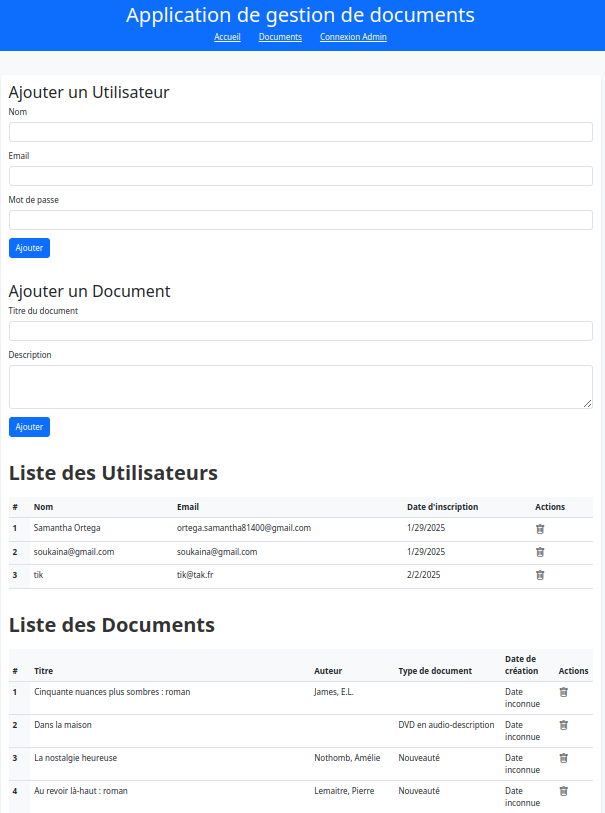
\includegraphics[scale=.8]{page_admin.png}}
		\caption{Page d'administration}
	\end{center}
\end{figure}

\newpage


\section{Témoignages des membres du groupe}

\subsection*{Hudayfa}

\say{\textit{Le plus compliqué était l'ajout des utilisateurs et des documents, surtout pour bien gérer les erreurs et les redirections. La connexion admin aussi, avec la vérification des identifiants et des sessions, ça m'a pris du temps. Au total, j'ai travaillé sur le projet à peu près 6h.}}

\subsection*{Hugo}

\say{\textit{Globalement, je n'ai pas ressenti de difficultés particulières dans les missions. Le plus compliqué a été de comprendre le fonctionnement de Mongoose pour construire le fichier \texttt{Document.js}. En tout, je pense que le projet m'a pris environ 5 heures.}}

\subsection*{Samantha}

\say{\textit{J’ai eu du mal à mettre en place les fonctionnalités d’emprunt et de retour. J’avais réussi à faire mes fonctions sans la page de connexion, mais l’intégration du token m’a posé problème pour récupérer l’ID de l’utilisateur et déterminer ce qu’il pouvait emprunter ou rendre. Au total, j’ai passé environ 4 heures sur le projet.}}

\subsection*{Soukaina}

\say{\textit{J'ai passé environ 2h30 sur le projet. J’ai eu du mal au début avec la connexion à la base de données. Je pensais devoir la configurer avec la mienne parce que je n’avais pas accès à celle d’Hugo, mais j’ai finalement découvert que celle de Hugo fonctionnait sans problème. \\
Pour les fonctions d’inscription et de connexion, ainsi que l’ajout des routes et des templates, ça ne m’a pas pris de temps du tout, car je les avais déjà faits en .NET, donc c’est la même logique.}}

\end{document}
